\documentclass[a4paper,12pt]{article}
\pagestyle{headings}
\usepackage[utf8]{inputenc}
\usepackage{aeguill} 
\usepackage{wrapfig}
\usepackage{graphicx}
\usepackage{gensymb}
\usepackage{fullpage}
\usepackage[spanish]{babel}
\graphicspath{ {project_proposal_img/} }
 


\begin{document}

\begin{titlepage}
\begin{center}

% Upper part of the page. The '~' is needed because \\
% only works if a paragraph has started.
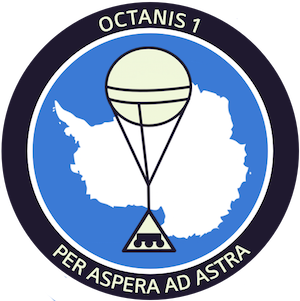
\includegraphics[width=0.35\textwidth]{patch}~\\[2cm]

\textsc{\Large Propuesta de Proyecto}\\[0.5cm]

% Title
\huge \bfseries Octanis 1: Unidad Robótica Autónoma Exploradora y Sistema de Transmisión de Datos vía Satélite en Tiempo Real de Bajo Presupuesto para la Antártida \\[0.4cm] 

\vspace{23pt}

\includegraphics[width=0.25\textwidth]{black_logo} \\
\vfill

% Bottom of the page
{\large \today} \\
\textsc{\small info@octanis.org | www.octanis.org}
\vspace{50pt}


\begin{table}[h!]
\centering
\vspace{1pt}
\begin{tabular}{ l  l  l }
	\textbf{Rev.} & \textbf{Traducciones} & \textbf{Autores} \\
	25.6.14 & Propuesta Inicial & Samir Sulaimanov, Raffael Tschui, Ana Roldán, Pamela Canjura \\
	27.6.14 & Versión en Español & Ana Roldán \\
	27.6.14 & Versión en Alemán & Raffael Tschui \\
\end{tabular}
\end{table}

\end{center}
\end{titlepage}

\tableofcontents

\pagebreak

\section{Introdución}
»octanis | exploración y descubrimiento« \cite{octanis} es una iniciativa estudiantil multidisciplinaria que nos embarca en un ambicioso y desafiante proyecto. La exploración polar. Como primer objetivo tenemos la creación de Octanis 1, un robot autónomo adaptado para resistir las condiciones extremas de las costas antárticas y al mismo tiempo realizar el estudio de las condiciones climáticas en el área. 
Octanis 1 transmitirá los datos obtenidos a través de sus sensores de temperatura, presión atmosférica, humedad relativa, posición y altitud en tiempo real.  Entre la información que se podría recopilar de manera facultativa están las concentraciones de diferentes gases en la atmósfera, los niveles de radiaciones $\alpha, \beta, \gamma$ e incluso muestras de hielo o nieve.  \\ Octanis 1 contara con una broca capaz de perforar el hielo \cite{krishnakant}. y extraer muestras que el mismo robot se encargaría de derretir con el fin de analizar su PH.
\\ La energía necesaria para el funcionamiento de Octanis 1, será suministrada por paneles solares ubicados sobre el robot en combinación con un paquete de baterías. La comunicación con el robot se realizara a través de la red de satélites Iridium  \cite{iridium}, que ademas de proporcionar una conexión económica y fiable desde cualquier punto del globo, exige una cantidad mínima de energía.


\section{Resumen de la Misión}

El objetivo de la misión Octanis 1, es construir una unidad robótica autónoma, mobil, de bajo presupuesto, y de bajo impacto ambiental que sea capaz explorar ambientes inhóspitos y realizar experimentos e investigaciones científicas y a la vez transmitir los datos obtenidos en tiempo real. El robot será pequeño y ligero, lo suficiente como para ser transportado por globos meteorológicos. Su diseño le permitirá transitar superficies congeladas y ser resistentes a las ráfagas de viento. Generará su propia energía a través de paneles solares y auto-regulará su temperatura interna, con el fin de optimizar el consumo de energía. El robot será una plataforma de tracción en cuatro ruedas, cada rueda estará conectada a un eje independiente, dando libertad de movimiento y orientación absoluta, incluyendo, levantarse y girar por completo.


\subsection{Objetivos}

Octanis 1 tiene como objetivo la construcción de un robot económico, de bajo impacto ambiental que tenga la capacidad de recopilar datos meteorológicos y ambientales bajo condiciones extremas en la Antártida. Todo esto con el fin de obtener datos fiables y en tiempo real sobre las condiciones en la Antartida. Esta información será publicada en tiempo real en la pagina www.octanis.org con el fin de que cualquier persona pueda realizar investigaciones o estudios con datos fiables y fácilmente accesibles.
Octanis 1 será un robot suficientemente pequeño y ligero como para ser transportado por globos meteorológicos. Ha sido diseñado especialmente para moverse sobre hielo y para resistir fuertes ráfagas de viento sin voltearse. El robot estará dotado de paneles solares y baterías para asegurar un suministro continuo de energía que le permita regular su temperatura y realizar todas las actividades y mediciones planeadas durante los meses de verano austral. Como sistema de tracción contará con cuatro ruedas conectadas a ejes independientes que dotarán a Octanis 1 de movilidad absoluta y la capacidad de girar sobre su propio eje y levantarse.


\paragraph{Robótica}
Su diseño en hardware y software ha sido concebido de manera simple pero funcional, resultado de un riguroso proceso de optimización en el que se buscaron materiales ligeros y resistentes a condiciones extremas incluyendo la presencia de agua, nieve y fuertes ráfagas de viento. El robot esta diseñado para cumplir sus misiones de manera autónoma o con mínima asistencia humana. Se programará un recorrido mediante puntos GPS y el robot tendrá la capacidad de evitar obstáculos y optimizar su velocidad. Toda comunicación con Octanis 1 será via la red de satélites Iridium. Gracias a la inclusión de paneles solares en su diseño, este robot podrá realizar misiones de varios meses de duración mientras dure el verano austral.

\paragraph{Sensores}
Todos los sensores estarán conectados al transmisor de datos, de modo que la información llegue a los usuarios de la forma mas rápida posible. Todos los datos recogidos por los sensores serán procesados y publicados en una interfaz estandarizada, de forma que en misiones futuras exista cooperación entre maquinas y estas puedan funcionar como un enjambre. 

\paragraph{Despliegue}
Se han analizado diversos métodos para el despliegue de esta misión, tomando en cuenta las dificultades de acceso y el aislamiento de los polos. Hasta este momento hemos dado con 2 alternativas: enviar a Octanis 1 en un globo meteorológico hasta la ubicación deseada y hacerlo descender usando un pequeño paracaídas o enviar una delegación de la organización para dejar el robot en el entorno a estudiarse. Los costos y riesgos de cada método deben ser analizados y discutidos en función del presupuesto y las probabilidades de éxito de de cada uno.


\paragraph{Libre \& Reproducible} 
Hemos diseñado el proyecto Octanis basándonos en los principios del movimiento de código abierto. Esto significa que todos los diseños, documentación, software y simulaciones 3D estarán disponibles al publico general en nuestro sitio web. Cualquier persona será libre de descargar, adaptar, reutilizar y distribuir esta información. Hemos hecho el esfuerzo de utilizar piezas y materiales fáciles de conseguir para que cualquier persona pueda replicar esta experiencia. También utilizamos técnicas de fabricación de bajo presupuesto como impresoras 3D, un fab lab  \cite{fablab} o un hacklab \cite{hackerspace}. El acceso a estas infraestructuras esta disponible para cualquier persona con un presupuesto mínimo.
 

\subsection{Programa}

El calendario se ha planeado para ser ejecutado en el 2014-2015 a menos que se nos indique lo contrario. Ciertas fechas precisas deben ser coordinadas en colaboración con el Instituto Antártico.  del Ecuador. Al estar ideado por un pequeño grupo de personas, este proyecto se gestiona de manera ágil y transparente. Además su desarrollo es cíclico con la finalidad de incorporar rápidamente cualquier modificación o mejora que pueda presentarse. Este metido ha funcionado de forma eficiente hasta ahora, dando una respuesta inmediata a los problemas o dificultades que han surgido. Toda la documentación es publicada regularmente a través de GitHub  \cite{octanisgithub} para que toda la gestión sea lo mas transparente posible. 

\begin{table}[h!]
\centering
\begin{tabular}{ l | l | l | c }

\bfseries{Código} & \bfseries{Fases de la Misión} & \bfseries{Fechas} & \bfseries{Semanas} \\
\hline
A1 & Diseño del Prototipo \& Desarrollo & 1.6. - 1.10. & 12 \\
A2 & Desarrollo de Software & 1.6. - 1.10. & 12 \\
B1 & Pruebas Iniciales & 1.10. - 14.10. & 2  \\
B2 & Unidad \& Toma de Muestras en el Glaciar Suizo & 14.10. - 14.11. & 4 \\
D & Prueba de Esfuerzo Mecánico  & 14.11. - 21.12. & 1 \\
E & Pruebas de Gestión Energética & 21.11. - 14.12. & 3 \\
F & Pruebas de Aterrizaje con Paracaídas & 14.12. - 21.12. & 1 \\
0.1 & Despliegue en la Antártida  & 14.2.2015 &  1 \\
0.2 & Despliegue en la Antártida  & 1.12.2015 &  1 \\

\end{tabular}
\caption{Linea de Tiempo del Despliegue.}
\end{table}

Una vez desplegada la misión, el programa continuará según la siguiente tabla. Los datos sobre el estado de la misión y autodiagnóstico de Octanis 1 serán enviados varias veces al día de forma automática. Los comandos para cancelar, pausar o modificar la misión podrán ser enviados en cualquier momento.

\begin{table}[h!]
\centering
\begin{tabular}{ l | l | c }
\bfseries{Código} & \bfseries{Fases de la Misión} & \bfseries{Semanas} \\
\hline

0 & Despliegue & 1 \\
1 & Chequeo y Comprobación de los Sistemas & 1 \\
2 & Unidad \& Muestreo & 3 \\
3 & Prueba de Cámara \& Transmisión de Imágenes  & 3 \\
4 (*)& Pruebas de Transmisión de Radio Amateur  & 3 \\

\end{tabular}
\caption{Linea de Tiempo de la Misión Científica.}
*Dependiendo de la ubicación y las estaciones de la base antártica, y la capacidad del despliegue radial.

\end{table}

\pagebreak

\subsection{Equipo de Trabajo}

Somos un grupo de estudiantes dispuestos a desafiar nuestros límites. Octanis 1 será construido por nosotros mismos, pero también contaremos con la ayuda y asesoramiento de profesores, consejeros y expertos que hemos conocido y conoceremos a lo largo del transcurso de la misión. Por lo tanto, quienes presentamos a continuación son el equipo principal:


\paragraph{Sam Sulaimanov} 
\begin{wrapfigure}{l}{0.2\textwidth}
    \centering
    \vspace{-13pt}
    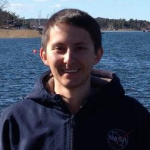
\includegraphics[width=0.15\textwidth]{sam}
\end{wrapfigure} tiene siete años de experiencia trabajando como programador e ingeniero en redes y  telecomunicación. Él ha estado trabajando con microcontroladores y sistemas electrónicos desde que era un niño y se encargará de que las funciones cerebrales de Octanis trabajen a la perfección.
\\ \\

\begin{wrapfigure}{l}{0.2\textwidth}
    \centering
    \vspace{-13pt}
    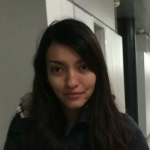
\includegraphics[width=0.15\textwidth]{ana}
\end{wrapfigure}
\paragraph{Ana Roldán} es una apasionada físico en entrenamiento y se encuentra involucrada en todas las areas de desarrollo del proyecto. Nunca se intimida ante los desafíos  y no tiene miedo de hacer las grandes preguntas e inspirar a todos con su intensa pasión por la Ciencia.
\\ \\

\begin{wrapfigure}{l}{0.2\textwidth}
     \centering
     \vspace{-13pt}
    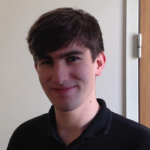
\includegraphics[width=0.15\textwidth]{raf}
\end{wrapfigure} 
\paragraph{Raffael Tschui} es un Ingeniero Eléctrico, EPFL, BSc. Tiene el vital papel de la generación energética, el control y la regulación del proyecto. Mantendrá el corazón de Octanis latiendo. Actualmente se encuentra en una misión en Colombia, como ayudante de un Profesor de la EPFL en la construcción de un bioreactor purificador de agua.
\\ \\

\begin{wrapfigure}{l}{0.2\textwidth}
    \centering
    \vspace{-13pt}
    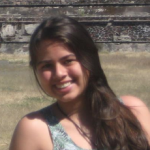
\includegraphics[width=0.15\textwidth]{pam}
\end{wrapfigure} 
\paragraph{Pamela Canjura}  su interés por la química despertó a los 5 años y no ha cesado desde entonces. Compitió varias veces en las Olimpiadas Internacionales de Química. Ella esta trabajando en los análisis químicos que serán hechos a bordo de Octanis.
\\ \\


\subsection{Presupuesto}

La siguiente tabla describe el presupuesto con precisión $\pm 20\%$ (c.p. = costos prioritarios): \\ 

\begin{table}[h!]
\centering
\begin{tabular}{ l | c || r }
  Costo de Artículos & Prioritarios & Gastos no Recurrentes \\
  \hline
  Energía Solar del Robot \& Calefacción & c.p. & 1150 USD \\
  Comunicación del Robot & c.p. & 570 USD \\
  Instrumentos del Robot \& Sensores & c.p. & 570 USD \\
  Electrónicos del Robot & c.p. & 790 USD \\
  Elementos Mecánicos del Robot \& Movilidad & c.p. & 1150 USD \\
  Transporte con el Globo & opc. & 1690 USD \\
  \hline \hline
  & & Costos Prioritarios: 4230 USD  \\
  & & Opcional: 1690 USD \\
\end{tabular}
\caption{Presupuesto General.}
\end{table}


El único costo recurrente es la transmisión satelital de Iridium \cite{iridium}. Este rango va desde 0.04-0.12 GBP por mensaje (340 bytes / Message-Out) y con una tarifa estándar de linea de alquiler de 8 GBP / mes. El costo por menaje depende de la cantidad de mensajes necesitados.



\section{Transporte y Despliegue del Robot}

Octanis 1 es un vehículo ligero lo que significa que su masa total no excederá de 2,5 kg. Gracias a esto, hay varias opciones de despliegue rentables disponibles, mismas que se enumeran a continuación:

\subsection{Métodos de Despliegue}

\begin{figure}[h!]
	\centering
    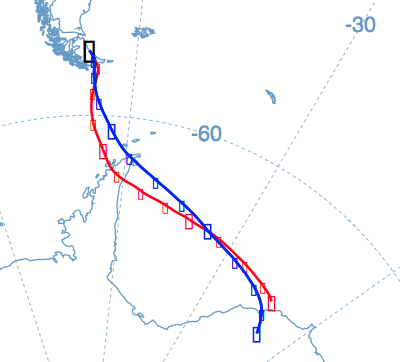
\includegraphics[width=0.4\textwidth]{trajectory}
    \caption{Simulación de una posible trayectoria desde Río Grande, Argentina con HYSPLIT.}
\end{figure}

\paragraph{Globos de Gran Altitud} o mas comúnmente conocidos, como globos climáticos. Uno puede ser usado para llevar al robot hasta su destino final. Llenos de Helio, estos normalmente flotan a una altura de 30 km y con una trajectororia asignada de cientos de kilómetros. Sin embargo la trayectoria a seguir del globo no puede ser controlada y depende de una rigurosa pre-simulación de vuelo hecha a través del simulador de software HYSPLIT  \cite{hysplit} \cite{hysplitjava}. Este es el método mas barato para enviar el robot a la Antártida, solo requiere como punto de partida algún lugar de america del sur, donde es posible tomar un vuelo comercial, y luego en la locación escogida dejar despegar el globo junto con el robot. Pero con este beneficio viene un alto riesgo de fallas en el despliegue. Incluso con modelos climáticos precisos, el clima podría cambiar repentinamente y sacar el globo de su trayectoria. Pero debemos aclarar que, HYSPLIT fue utilizado con éxito en numerosos proyectos de este tipo, como  el Orbitador Breitling de Piccard y Jones 3 \cite{hysplitexamples}.
Una vez que el robot y el globo hayan llegado a su destino final, el robot se separa del globo y aterrizará con la ayuda de un paracaídas. El globo continuará divagando sin trayectoria fija, hasta que finalmente explote o caiga al suelo cuando el helio se haya dispersado.

\begin{figure}[h!]
	\centering
    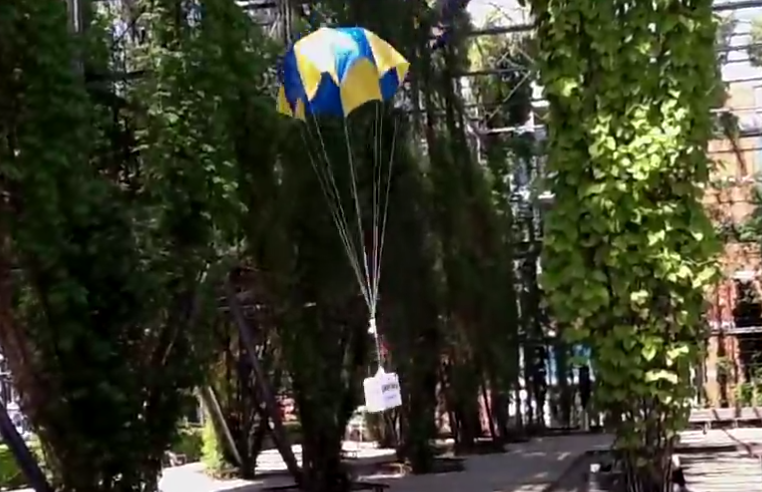
\includegraphics[width=0.5\textwidth]{lowcostchute}
    \caption{Fotografía de una prueba de aterrizaje con un paracaídas de bajo costo, fabricado por el equipo de Octanis.}
\end{figure}


\paragraph{Helicóptero} - un método a considerar es desplegar Octanis desde un helicóptero que ya se encuentra en una ruta específica. El rover se podría dar a uno de los pasajeros o conectarse al cable de transporte, separándose en el momento adecuado. Al igual que en el despliegue con el globo, Octanis aterrizaría rápidamente en paracaídas y estaría listo para comenzar su misión.


\paragraph{Manual} este despliegue se sugiere cuando los costos y los riesgos necesitan ser los más bajos posibles. Este es, con mucho, el método más fácil, simplemente se debe ir a la ubicación deseada y ajustar el robot para que empiece su exploración. Octanis continuaría por sí mismo y regresará a la localización deseada.



\subsection{Sustentabilidad Ambiental}
Es conveniente no dejar residuos, siguiendo los requerimientos del Tratado Antártico. Dependiendo variación del método de despliegue, la masa total y el tipo de materiales que se incluirían en una misión a la Antártida. Un despliegue del robot a un objetivo fuera del alcance de las expediciones antárticas normales, se realizaría mediante el uso de un globo de gran altitud, con una masa de 3 kg, hecho de látex utilizado por los globos meteorológicos estándar. En una misión de larga distancia, el robot se separará del globo en el lugar de destino y el globo continuará flotando sin supervisión. Por lo tanto, no tendríamos con precisión el lugar de aterrizaje del globo. Debido a la naturaleza de este tipo de misiones en particular, por lo general el robot sería irrecuperable, convirtiendose en una pequeña base fija que recopilaría información constantemente del lugar.

En un primera fase, se propone, por lo tanto seleccionar un lugar de aterrizaje que este al alcance de las expediciones o bases antárticas normales. Incluso es posible liberar el robot por otros medios, llevándolo a la ubicación de forma manual o por medio de helicóptero.

Concluyendo, el robot está construido de polímeros y metales, y existe un mínimo  riesgo de que este se salga de control debido a una falla de funcionamiento. La masa total robot, sin embargo no excede los 2,5 kg, por lo que la contaminación producida es mínima. En el improbable caso de avería, el vehículo puede recuperar de forma manual siguiendo la última ubicación conocida a través de las transmisiones.




\section{Subsistema del Robot}

\subsection{Ordenador a Bordo}
\begin{figure}[h!]
	\centering
    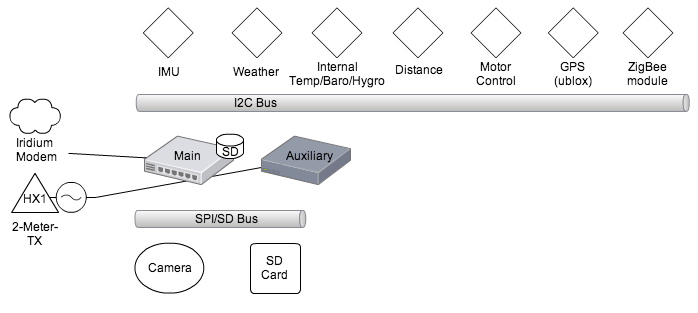
\includegraphics[width=1\textwidth]{schema}
    \caption{Esquema del sistema informático a bordo de los periféricos.}
\end{figure} 
La familia de microcontroladores de 16 bits de potencia ultra baja, Texas Instruments MSP430, es la opción preferida para ser el procesador de sistema informático integrado del robot. El microcontrolador se hará cargo de la mayoría de las tareas de control y regulación, la trayectoria específica, la navegación, las comunicaciones y los sensores de procesamiento. El sistema ejecutará un sistema operativo en tiempo real, capaz de realizar múltiples tareas, diferenciando las tareas prioritarias. El equipo va a interactuar con los siguientes periféricos a bordo:

\begin{itemize}
\item Unidad de Medida Inercial: acelerómetro, giroscopio, magnetómetro, barómetro de precisión.
\item Módulo de tiempo: temperatura, barómetro, higrómetro, anemómetro.
\item Instrumento Científico: Sonda de pH.
\item Módulo Óptico: cámara, Sensores de distancia.
\item Modulos de Desplazamiento: controladores de motores, sensores de corriente.
\item Communicación: Iridium, APRS, ZigBee.
\item Tarjeta de Memoria SD.
\item Módulo GPS.
\end{itemize}

Un ordenador auxiliar estará disponible si el ordenador principal falla. Este tratará de reiniciar el ordenador principal y si no lo consigue proporcionará la funcionalidad básica del sistema.



\subsection{Fuentes de Energía}

La energía de la luz solar por metro cuadrado es $E_0*sin(\alpha)$ con $E_0=1367 W/m^2$ \cite{solarc} y $\alpha$  es el ángulo de los rayos que caen y el eje horizontal. Para la Antártida, podemos usar $\alpha \approx 23.5+90+|\phi|$ donde $\phi$ es la latitud, para obtener un estimado de la máxima energía disponible (es decir en verano) en un determinado punto geográfico (see fig. 4).


\begin{figure}[h!]
	\centering
    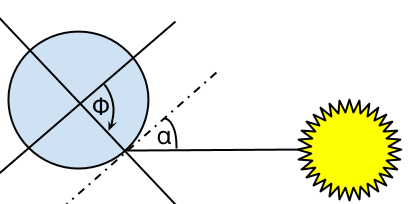
\includegraphics[width=0.6\textwidth]{sun}
    \caption{Concepto de diseño de Octanis, basado en el nanorobot MUSAS-CN}
\end{figure}


Esto llevaría a $1050 W/m^2$ para el punto más septentrional de la Antártida(@ 65\degree S) y $545 W/m^2$ en el polo sur (@ 90\degree S). Hay que tener en mente que durante los 6 meses de verano, este valor oscilará entre 0 y el máximo valor calculado\cite{pvedu}. 
Asumiendo que nuestros paneles están instalados horizontalmente y considerando la eficiencia de los paneles solares (alrededor del 15-20\%)  esto significa que por metro cuadrado podremos convertir max. 200 W en energía eléctrica. Si calculamos con una eficiencia pesimista y una "radiación de valor medio" durante los 6 meses de la misión (sólo 1/2 del valor máximo), necesitaríamos un panel cuyo tamaño sea de $0.13m^2$ (@ 65\degree S) to $0.25m^2$ (@ 90\degree S) para obtener 10 W de potencia.Pero sin  considerar la oscilación diaria del ángulo de la radiación, o que hay ciertos periodos de penumbra. Por lo tanto, es más razonable usar los valores obtenidos en base a la segunda opción $0.25m^2$ (también tomando en cuenta que la energía que podemos suministrar decrece con el mal clima).

Para resumir, la superficie de un panel de $0.25m^2$ proveería en promedio (estacional, diario) una potencia de 10W, siendo estos números proporcionales. 


\subsection{Procesos Térmicos}

La máxima prioridad es mantener el sistema a -20\degree C o superior, lo que significa que toda la energía de los paneles solares y, si es necesario, de la batería, se utilizará primero para mantener una temperatura en la que los sistemas funcionen adecuadamente. Por lo consiguiente, el sistema de calefacción estará conectado directamente entre los paneles solares y el controlador de carga de la batería. Se controlará a través de comparadores electrónicos que escogen una u otra fuente de energía para alimentar las almohadillas de calor en función de los umbrales de temperatura específica que se indican a continuación. El controlador de carga en sí se ocupa de los límites de temperatura para la alimentación de la batería y se enciende y apaga automáticamente. 


\subsection{Procesos Mécanicos}
El diseño del cuerpo del robot (fig. 5) ha sido sustancialmente influenciado por el nanorobot de la NASA MUSES-CN \cite{muses}. Este es un diseño único, que permite la libertad casi completa de movimiento. Hemos diseñado Octanis 1 para que sea ligero, con una área superficial lo suficientemente grande para producir la energía solar que se necesita durante de la misión. Las dimensiones de la carrocería son aproximadamente 30cm x 30cm x 6cm.

\begin{figure}[h!]
	\centering
    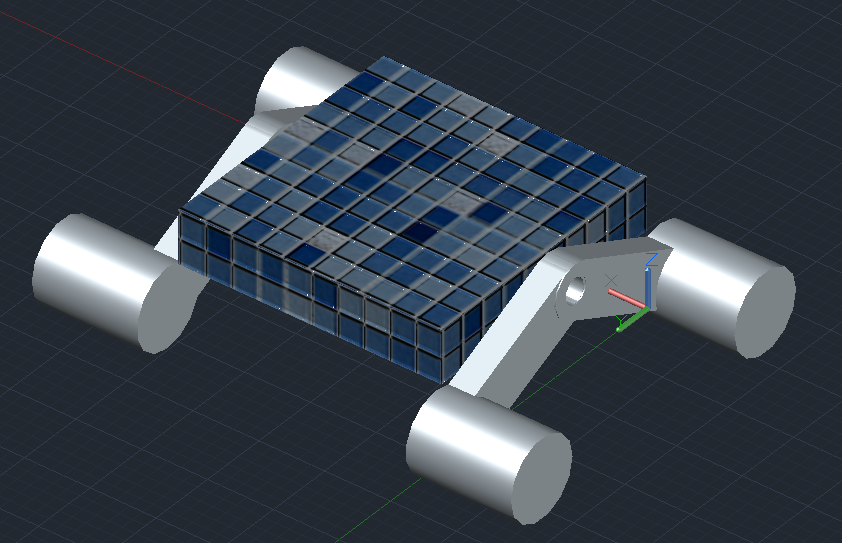
\includegraphics[width=0.5\textwidth]{conceptrover}
    \caption{Concepto de diseño de Octanis, basado en el nanorobot MUSAS-CN.}
\end{figure}

Como podemos observar en la figura 6, este diseño permite al robot cambiar de orientación dependiendo de los requerimientos de la situación. Siendo las principales preocupaciones de la misión, el suministro de energía y la resistencia a la intemperie. Y dado a que todo el cuerpo del robot está cubierta de paneles solares, este puede enderezarse de acuerdo a la posición del sol para exponer la mayor parte de su superficie a la luz solar. Esta capacidad también es crucial en condiciones climáticas adversas para asegurarse de que la nieve no cubra los paneles girando o volteando periódicamente al robot. No sólo la nieve, también el viento puede ser un problema, puede llegar a tumbarlo o ponerlo en una posición desfavorable. Si esto ocurriese, el vehículo podría volver a la posición de conducción adecuada mediante la activación de los puntales. Todos los apoyos de las ruedas se pueden girar alrededor de los ejes y están equipadas individualmente con un motor independiente. Estos se mueven a través de un tornillo con el fin de mantenerlas estáticas cuando no están girando sin tener que aplicar una fuerza constante. \\
Otra ventaja de este diseño es que podemos utilizarlo en la construcción de los dispositivos de perforación, haciendo este proceso más simple y eficiente. Mientras se perfora un núcleo de hielo, el robot puede descender, generando una fuerza adicional, su peso, como presión sobre el taladro. La broca sólo tiene que girar y no necesita retraerse en el cuerpo del robot.

\begin{figure}[h!]
\centering
\begin{tabular}{ c  c  c }
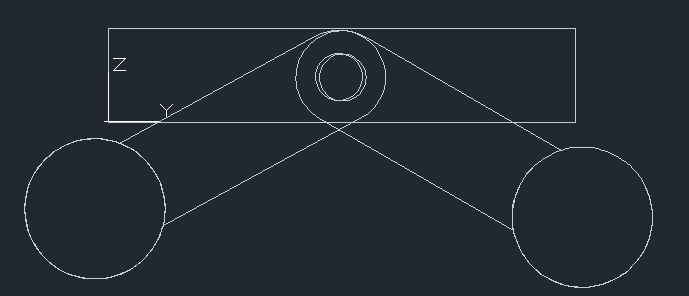
\includegraphics[width=0.3\textwidth]{drive} & 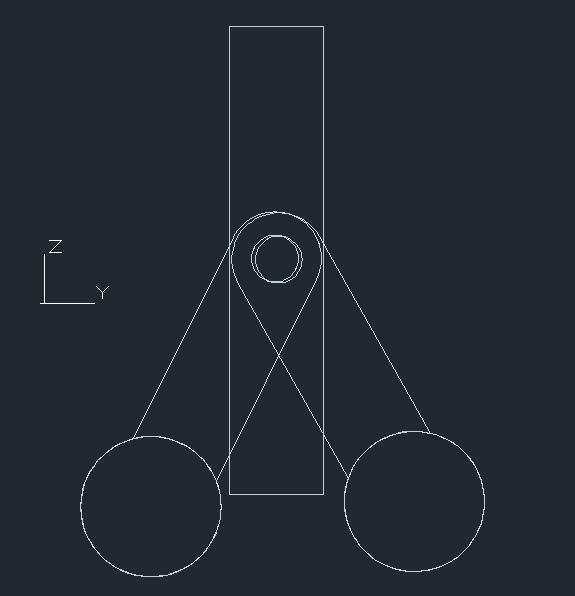
\includegraphics[width=0.25\textwidth]{upright} & 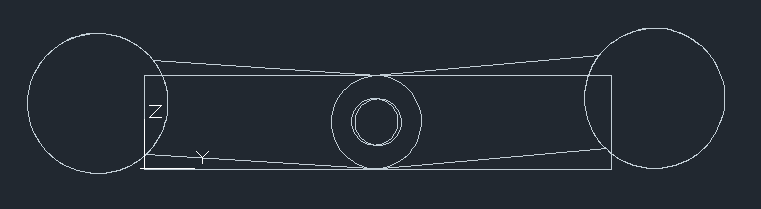
\includegraphics[width=0.4\textwidth]{flat} \\
\end{tabular}
\caption{Diferentes configuraciones de apoyo en las ruedas l.t.r.: (1) modo desplazamiento, (2) modo recarga solar, (3) modo a prueba de viento.}
\end{figure}


\subsection{Movilidad}
Un terreno cubierto de nieve y hielo será el principal hábitat Octanis por lo tanto las ruedas fueron diseñadas específicamente para este ambiente, con una superficie amplia, pero siendo ligeras, proporcionando una buena tracción en el ascenso. 
Las cuatro ruedas estarían motorizadas de forma individual proporcionando el impulso suficiente par para mover Octanis en una inclinación de 30 grados. Para realizar diferentes tipos de giros, la rotación de las ruedas en cada lado puede hacerse a diferentes velocidades.

\begin{figure}[h!]
	\centering
    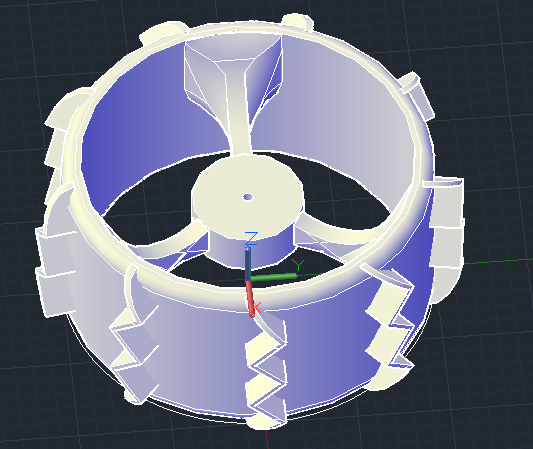
\includegraphics[width=0.4\textwidth]{wheel}
    \caption{Diseño de las ruedas inicial. Las aletas que sobresalen permiten que las ruedas excaven en la nieve durante el desplazamiento con una mejor tracción.}
\end{figure}


La unidad de medición inercial (IMU) se utiliza para conocer la orientación robot en cualquier momento. Está compuesta de un giroscopio, acelerómetro, barómetro de precisión y magnetómetro. La información de los sensores se retro-alimenta a los sistemas de control que activan los motores. En caso de que el vehículo tenga que ir sobre un obstáculo, los apoyos de rueda se pueden girar en la medida de lo posible de manera que el cuerpo del robot este siempre en un plano de orientación paralelo al suelo. Esto minimizará el riesgo de volcamiento y nos permitirá ir fácilmente sobre obstáculos mas grandes que el radio de la ruedas, de forma similar al sistema de suspensión rocker-bogie utilizado en vehículos de exploración de Marte de la NASA\cite{rockerbogie}. Debido al alto riesgo de vuelco causado por las ráfagas de viento, el diseño sin motor del rocker-bogie no fue seleccionado, ya que no hay una forma sencilla de ponerlo en pie si este llega a voltearse.

La velocidad máxima Octanis se estima en 100cm/min. Sin tener en cuenta la disponibilidad de energía en función de tiempo, esto le da un rango de alcance diario de aproximadamente 1 km. Habrá dos modos de desplazamiento: exploración y la ruta más corta. \textbf{Modo Exploración} hará que el robot atraviese con un amplia área de barrido una localización pre-seleccionada o busque un fenómeno específico \textbf{La ruta más corta} trae a Octanis desde una ubicación a otra a través del camino mas corto. Ambos métodos pueden utilizarse en combinación. Los obstáculos detectados pueden ser almacenados como puntos de referencia, lo que ayudaría a construir un mapa aproximado de la zona explorada.

\subsection{Sistemas de Comunicación}
La transmisión de datos con regularidad es una característica prioritarias de la misión del robot. Esto se logrará mediante el uso del servicio de transmición de datos a través del Iridium Short Burst (SBD) con la ayuda del módem RockBLOCK Iridium 9602 \cite{iridium}. Este módem permite la transmisión de paquetes de datos, con un máximo de envío de hasta 340 bytes y una recepción 270 bytes aproximadamente cada 20 segundos. Un conjunto de datos de mayor tamaño puede ser fragmentado y transmitido en varios paquetes. La conexión a este módem y a esta red está disponible en cualquier parte de la Tierra en cualquier momento, algo que no se puede decir de la red GSM o incluso de la radio amateur. El módem requiere igual de baja potencia como los GPS a bordo se suma a la lista de beneficios. La información enviada a través de la red Iridio se manda automáticamente a un servidor y se carga directamente en el sitio web del proyecto, donde el público puede ver el estado y los datos recopilados por Octanis.

Octanis 1 también estará equipado con un transmisor APRS unidireccional de 5 vatios, los sensores transmiten datos y la información de localización en una banda de 2 metros. Esta puede ser recibida por los operadores de radio amateur (o personas sin licencia con escáneres de radio) que se encuentren en este rango. El rango de este transmisor es normalmente de cientos de kilómetros cuando se envía directamente desde el cielo (es decir, conectada a un globo). Sobre el terreno, el rango es mucho menor.


\subsection{Sistemas Ópticos}
Octanis podrá tomar instantáneas según se le ordene, aunque con una cámara de baja resolución. Esto forma parte de un experimento que pretende averiguar si una imagen se puede enviar de manera eficiente a través de la red de Iridio. Además nos gustaría probar el procesamiento de imágenes a bordo (por ejemplo, la detección de características simples). El sistema óptico se completa con sensores de distancia que pueden detectar obstáculos más cercanos. Se evaluará si el LIDAR Neato XV-11 \cite{lidar} puede ser usado o si debemos utilizar sensores de distancia IR.


\subsection{Instrumentos Científicos}
El instrumento científico fundamental para esta misión es un taladro de hielo fusionado a una sonda de pH. El taladro será capaz de perforar un área de 1cm x 5cm en el hielo o nieve, retraerse desde la superficie fría y luego fundir la muestra. La muestra liquida de hielo o nieve sería analizada con una sonda de pH, un electrodo de vidrio, que determinará la acides de la muestra. Con el fin de minimizar los costos de la misión, en el sensor que se utilizaremos no es de alta calidad, y la precisión no puede ser garantizada por el fabricante. por lo que requiere ser calibrado, modificado y probado por nosotros. Suponemos que el dispositivo nos dará lecturas bastante precisas si se hace una comparación entre un gran número de muestras.

\pagebreak

\section{Conclusión}
Sabiendo que está es una misión ambiciosa y que el camino esta lleno de desafios, creemos que es un proyecto viable y factible. Cuando seamos alcancemos nuestros objetivos, seremos capaces de ofrecer a la comunidad científica (incluyendo a los llamados ciudadanos científicos) una plataforma móvil universal y adaptable. Que es capaz de soportar el hostilidad de la Antártida o ambientes similares.\\

Esperamos fascinar e inspirar a estudiantes, profesores, artistas, empresarios, científicos y al público en general para que compartan junto a nosotros esta investigación interdisciplinaria, despertando así el interés del público en la Ciencia e Ingeniería, con la esperanza de que todos se unan a nosotros en nuestra misión prioritaria, construir un mundo mejor.


\pagebreak
\pagestyle{empty}
\begin{thebibliography}{14}


\bibitem{krishnakant}
  Krishnakant Babanrao Budhavant, Pasumarthi Surya Prakasa Rao, Pramod Digambar Safai,
  \emph{Chemical Composition of Snow-Water and Scavenging Ratios over Costal Antarctica}.
  Aerosol and Air Quality Research, 14: 666–676, 2014.

\bibitem{octanis}
{\em »octanis | discovery and exploration« website} http://octanis.org, 23.6.2014.

\bibitem{iridium}
{\em Rock7 RockBLOCK website} http://rockblock.rock7mobile.com/products-rockblock.php, 25.6.2014.


\bibitem{octanisgithub}
{\em Octanis 1 GitHub repositories website} http://github.com/octanis1, 25.6.2014.

\bibitem{muses}
  Brian H. Wilcox, Ross M. Jones, 
  \emph{The MUSES-CN Nanorover Mission and Related Technology}.
  IEEE Aerospace 2000 Conference, 18.3.1999.


\bibitem{rockerbogie}
  Hayati, S., et. al., 
  \emph{The Rocky 7 Rover: A Mars Sciencecraft Prototype}.
  Proceedings of the 1997 IEEE International Conference on Robotics and Automation, pp. 2458-64, 1997.

\bibitem{hysplit}
  {\em HYSPLIT - Hybrid Single Particle Lagrangian Integrated Trajectory Model }, NOAA, http://www.ready.noaa.gov/HYSPLIT.php, 23.6.2014.

\bibitem{hysplitjava}
  {\em JAVA software to run multiple HYSPLIT simulations to find the optimal parameters for a trajectory}, http://github.com/octanis1/OctanisHYSPLIT, 23.6.2014.

\bibitem{hysplitexamples}
	{\em Ballooning with HYSPLIT}, \\
	http://www.arl.noaa.gov/documents/workshop/Spring2010/Balloon\_flights.ppt, 23.6.2014.

\bibitem{fablab}
	{\em Fab lab definition}, \\
	http://en.wikipedia.org/wiki/Fab\_lab, 25.6.14.

\bibitem{hackerspace}
	{\em Hackerspace definition}, \\
	http://en.wikipedia.org/wiki/Hackerspace, 25.6.14.

\bibitem{pvedu}
	{\em Effect of Light Intensity}, \\
	http://www.pveducation.org/pvcdrom/solar-cell-operation/effect-of-light-intensity, 25.6.14.

\bibitem{lidar}
	{\em Neato XV-11 LIDAR / Piccolo Laser Distance Sensor}, \\
	http://xv11hacking.wikispaces.com/LIDAR+Sensor, 25.6.14.

\bibitem{solarc}
	{\em Solar constant}, \\
	http://en.wikipedia.org/wiki/Solar\_constant, 25.6.14.

\end{thebibliography}

\end{document}